\documentclass[tikz]{standalone}
\usepackage{amsmath}
\usepackage{amssymb}
\usepackage{amsfonts}
\usepackage{tikz}

\thispagestyle{empty}
\begin{document}
\definecolor{nblue}{rgb}{0.40, 0.598, 0.83}
\definecolor{nred}{rgb}{0.9, 0.65, 0.675} 
\definecolor{n}{rgb}{0,0,0} % aka black 

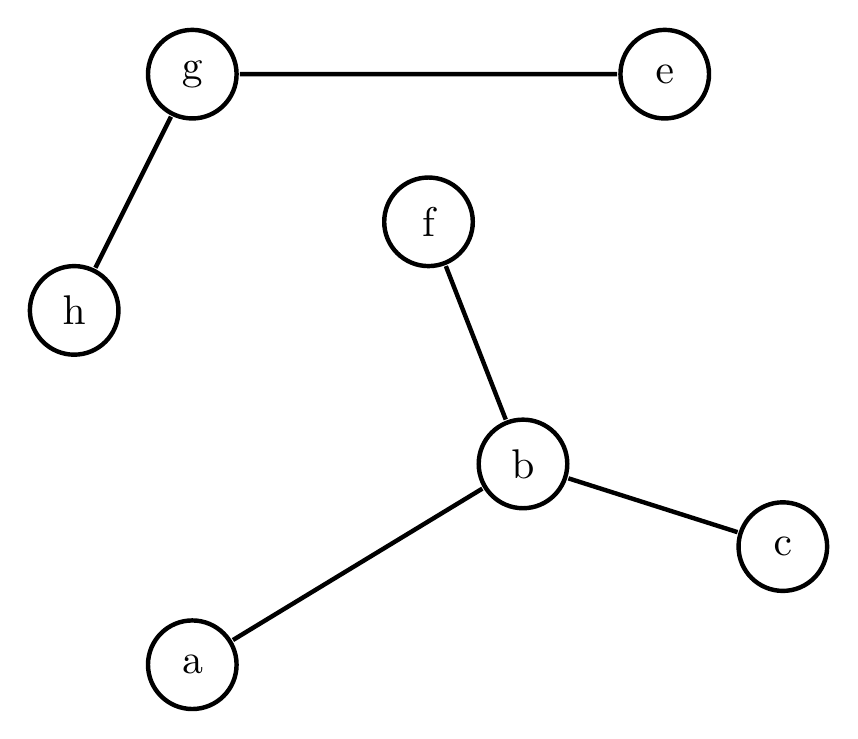
\begin{tikzpicture}[ultra thick, scale=1.5, transform shape, every node/.style={draw, circle, minimum size=.75cm}]
\node (a) at (0,0) {a};
\node (b) at (2.8,1.7) {b};
\node (c) at (5,1) {c};
%\node (d) at (6,3) {d};
\node (e) at (4,5) {e};
\node (f) at (2,3.75) {f};
\node (g) at (0,5) {g};
\node (h) at (-1,3) {h};

\draw (a) -- (b);
\draw (b) -- (c);
%\draw (c) -- (d);
%\draw (d) -- (e);
%\draw (e) -- (f);
%\draw (f) -- (g);
\draw (g) -- (h);
\draw (e) -- (g);
\draw (b) -- (f);

\end{tikzpicture}

\end{document}
